\chapter{Amplifier Circuits}
\textit{Amplifiers circuits} \cite{amplifier-circuit} are circuits which increases an electrical input signal according
to a specific transformation function (gain) for each different topology on the output. The circuit for small input signals
normally is composed by an operational amplifier, resistors, trimmer potentiometers to adjust the gain and capacitors.\\

It was required by the project an amplifier which have a gain of 100 ad should be possible to supply with a sigle supply, ideally 5V provided by
the USB port. The circuit should be compact to be a product differential, when compared to the existent systems which needs to connect on greater modules
to perform the same action as the proposed on this project.

It was researched some types of amplifiers circuits on \textit{book} \cite{Milmann} and on \textit{supplier catalogue} \cite{OpAmps}.
After verify some amplifiers topologies it was selected two different circuits which attends the project requirements.
The first circuit uses the Texas Instruments INA 326
Instrumental Amplifier and the second uses the Texas Instruments TLV 4316 Operational Amplifier. These topologies are possible to use with
single supply of 5V and the reach the desirable gain value without distortion on the project frequency range of work (audible frequency range).

\section{INA 326}
\label{INA_Circuit}
The project using the INA 326 IC, started with a research at the \textit{component datasheet} \cite{INA326}
of this component and the \textit{supplier catalogue} \cite{OpAmps}. On theses documents it was verified
the circuit topology \autoref{INA_topology} which provides the desired Gain to
the electric signal from the pickup respecting the project's initial requests.

\begin{figure}[!htpb]
\centering
\caption{INA 326 topology}
\label{INA_topology}
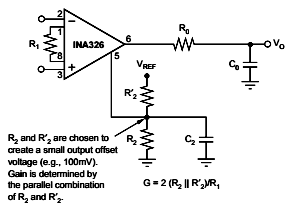
\includegraphics[scale=1]{images/Texas_INA}
\legend{Source: \citeonline{INA326}}
\end{figure}

This circuit amplifies the input signal and the gain is obtained by the \autoref{INA_Gain} provided by the \textit{component datasheet}
\cite{INA326}:

\begin{equation}
\label{INA_Gain}
G=2*\frac{(R_2||R_2 ')}{R_1}
\end{equation}

On the project the Resistor $R_0$ and the Capacitor $C_0$ was excluded because
it was not relevant on the output to this project. It was calculated the values
for the components and then developed a schematic model to perform some simulation tests
to verify the functionalism of the circuit for the desired application.
The schematic circuit \autoref{INA_Schematic} was developed using the software CadSoft Eagle Professional 7.6.0
until the final version.

\begin{figure}[!htpb]
\centering
\caption{INA 326 Schematic Circuit}
\label{INA_Schematic}
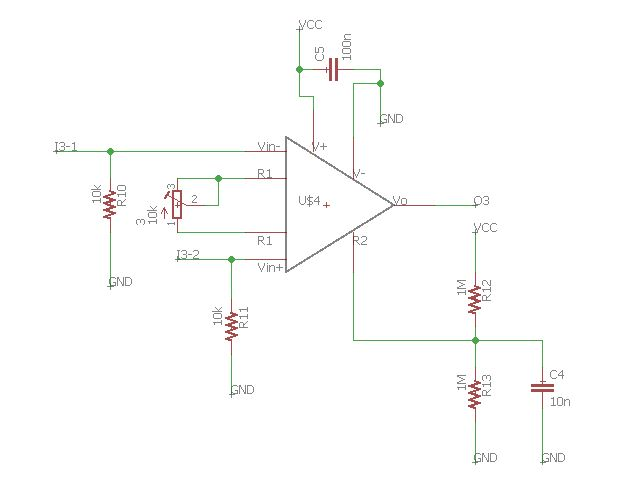
\includegraphics[scale=0.65]{images/INA_Schematic}
\legend{Source: made by authors}
\end{figure}

It was decided to use trimmer potentiometers on the amplification circuit to be possible perform small and precise adjustments to each
channel. These adjustments was on order to warranty the best relation of the gain to the channels.

Using the components values showed on the circuit \autoref{INA_Schematic} it was calculated
the Gain of the circuit. Using the trimmer potentiometer it was adjusted the gain value to the desirable value
of 1800.

The amplifier circuit was projected to each channel as showed on \autoref{INA_Complete}.
So the circuit needed 6 IC INA 326 to be complete.  After project
the schematic circuit to each channel it was developed the PCB project, using the
same software described on the schematic modeling. The PCB project \autoref{INA_PCB}\\


This PCB project \label{INA_PCB_doc} was projected on a dual layer board scheme, using 15 mils of
minimum width for the conductive tracks. It was assembled on FR4 dual layer copper
board, combining the through-hole and surface-mount technologies. This choice was
made due the facility of the assembly of the through-hole components and the availability
of the IC only on surface (SOP-8) encapsulation. It was sent
the files section nameto one person who works with printing PCB boards. After the processes
the PCB was like showed on \autoref{PCB}.\\

On this project it was used:

\begin{itemize}
\item 6 Instrumental Amplifiers INA 326;
\item 6 10k$\Omega$ Trimmer Potentiometer;
\item 6 10nF Ceramic Capacitor;
\item 6 100nF x 50V Electrolytic Capacitor;
\item 12 10k$\Omega$ $\frac{1}{4}W$ 5 Percent Tolerance Resistor;
\item 12 1M$\Omega$ $\frac{1}{4}W$ 5 Percent Tolerance Resistor;
\item 1 6 positions Pin bar;
\item 1 12 positions dual track Pin bar;
\item 1 2 positions Pin bar;
\end{itemize}

\begin{figure}[!htpb]
\centering
\caption{Projected INA PCB}
\label{INA_PCB}
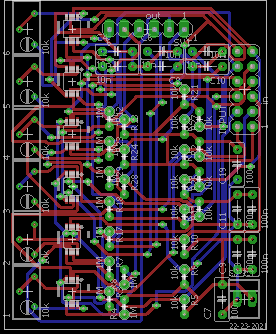
\includegraphics[scale=1.5]{images/TCC_INA}
\legend{Source: made by authors}
\end{figure}

\begin{figure}[!htpb]
\centering
\caption{PCB Project}
\label{PCB}
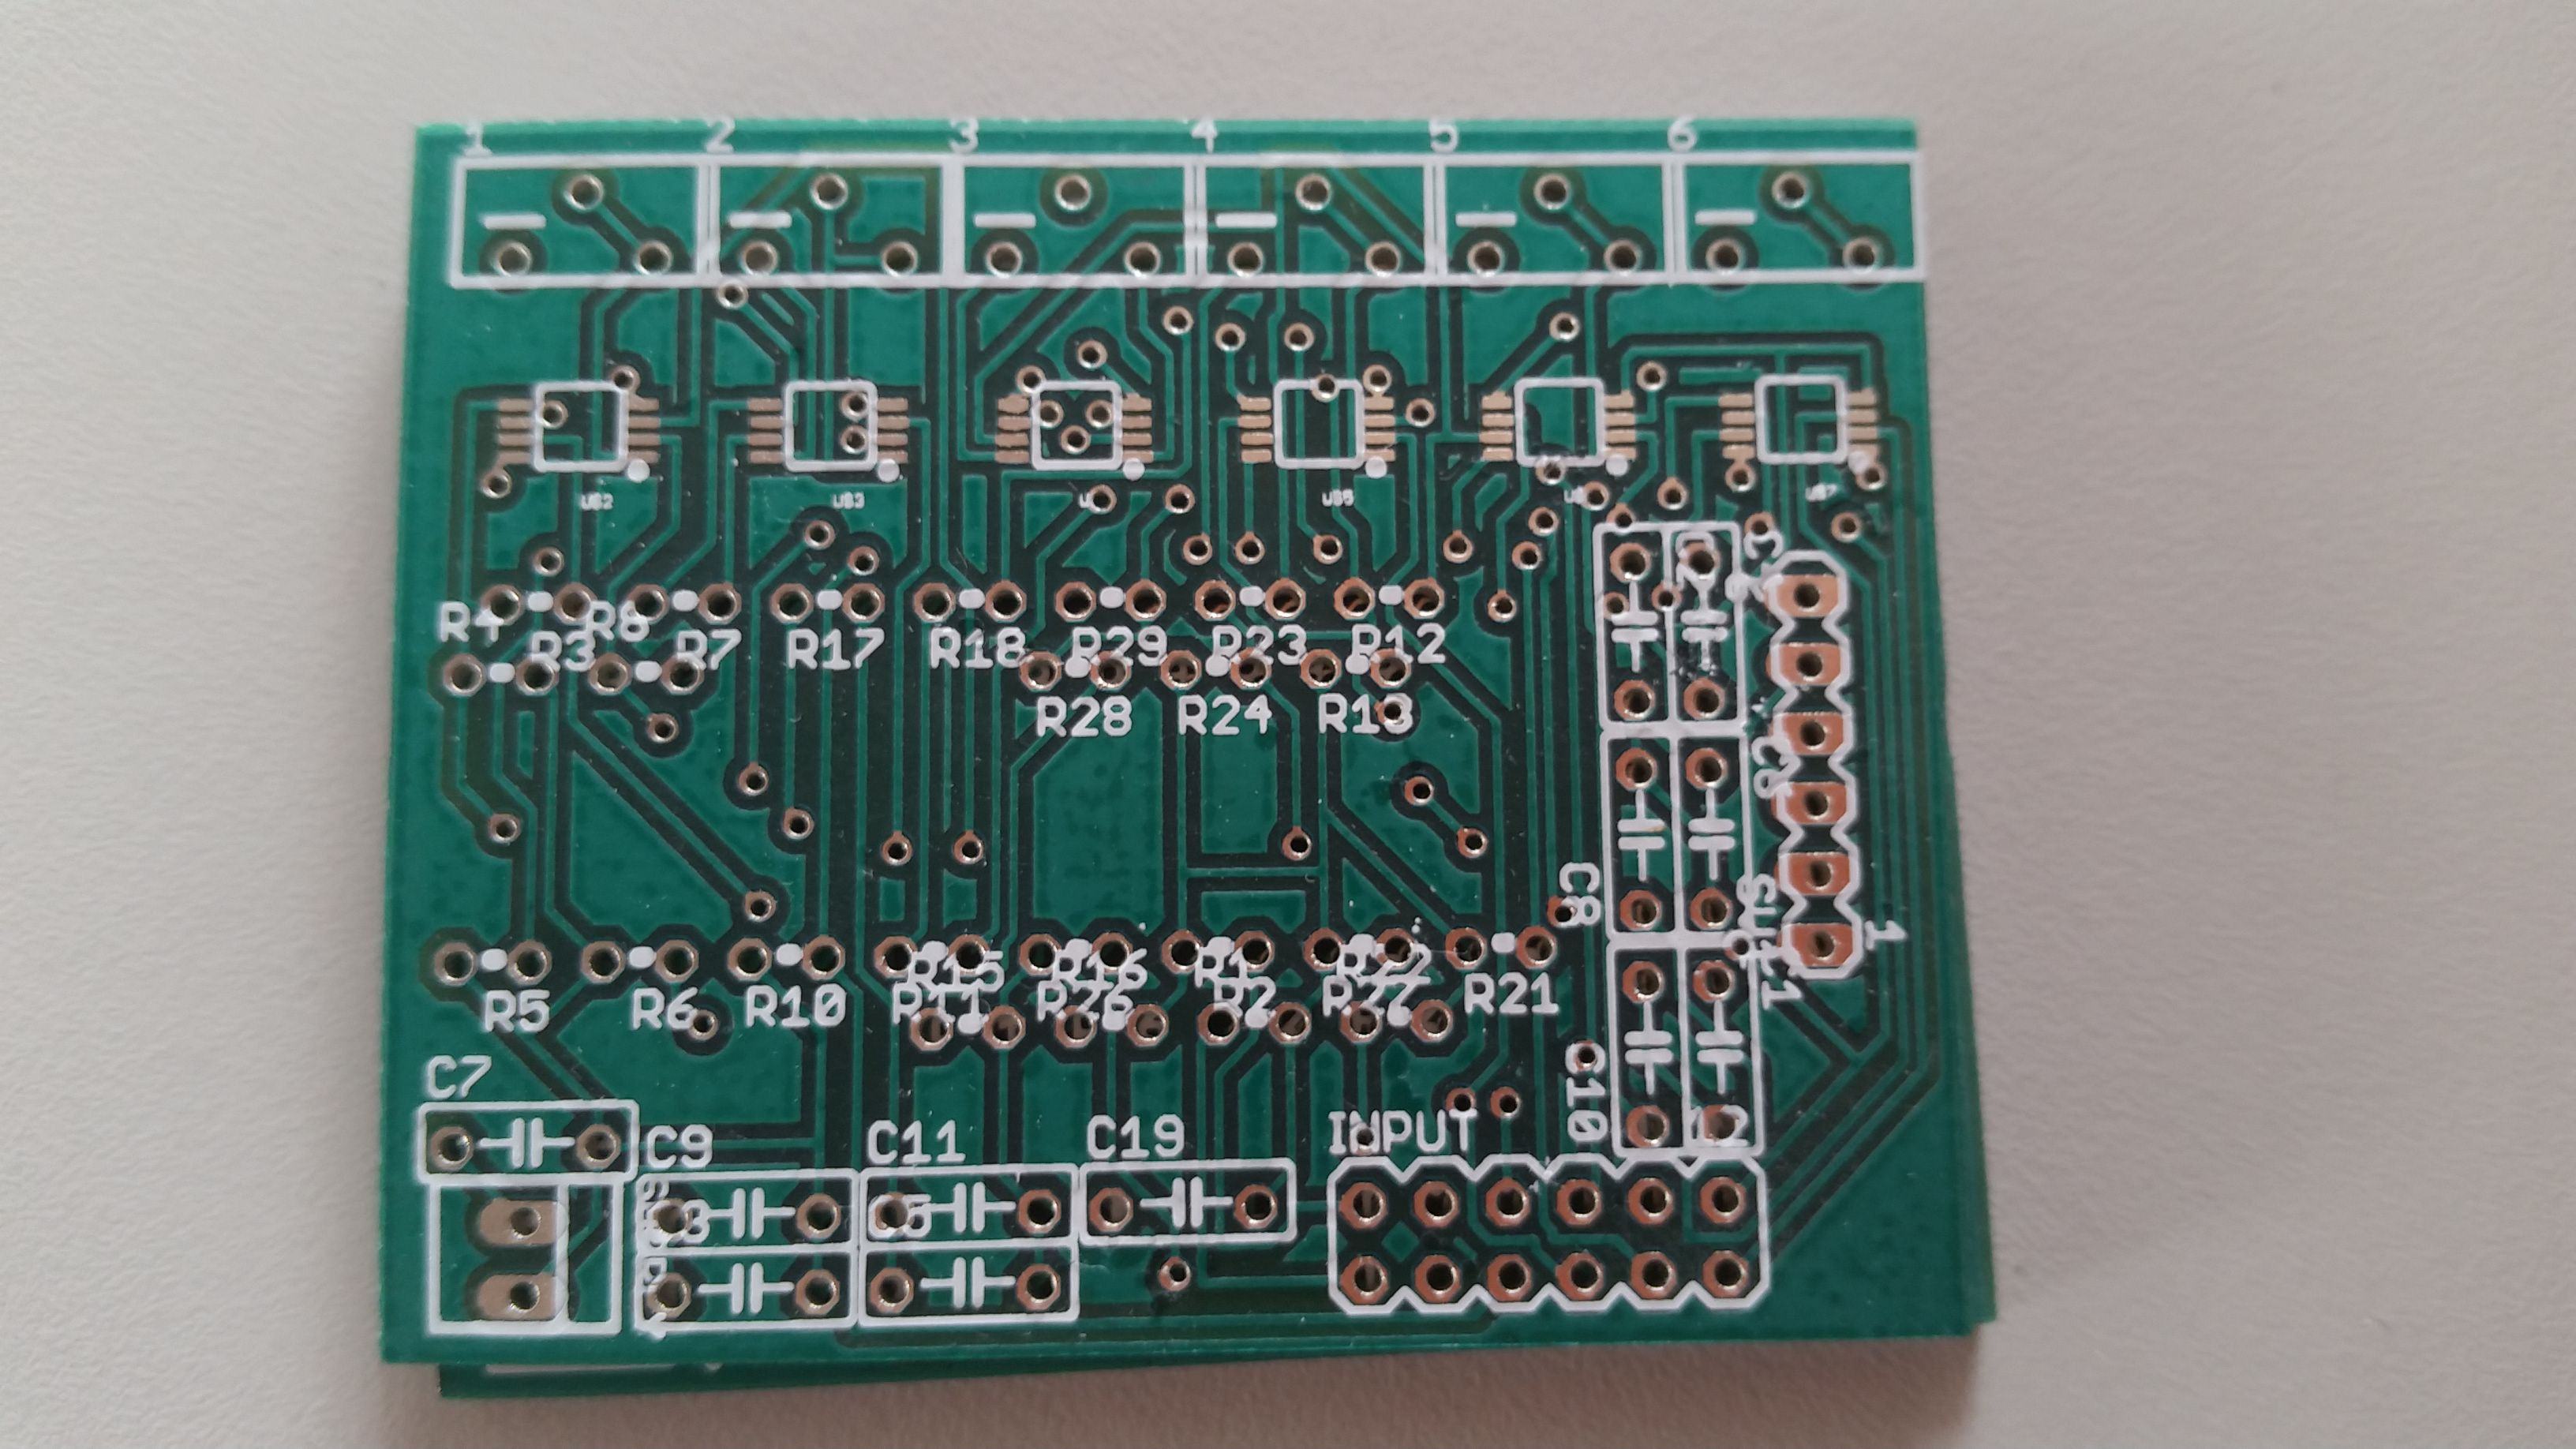
\includegraphics[scale=0.08]{images/INA_board}
\legend{Source: made by authors}
\end{figure}

After soldering all the components it was performed some bench tests to
verify the functionality of the amplifier circuit. The result showed that the
circuit attends the required function, amplifying the signal from a pick of 10mV
to a pick of 1V, proving that the circuit is working perfectly and attending the
demand of the project. After the bench test the system was connected to the pickup
to verify if the guitar signal would be amplified as needed to the conversion process.
The result was satisfactory and attended well the purpose to the project, as showed on \autoref{INA_result}.

\begin{figure}[!htpb]
\centering
\caption{Amplified pickup signal with INA circuit}
\label{INA_result}
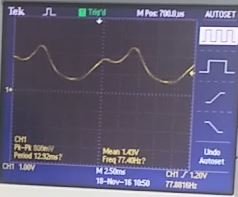
\includegraphics[scale=1]{images/INA_result}
\legend{Source: made by authors}
\end{figure}

\section{TLV 4316}
\label{TLV_Circuit}
The circuit using TLV 4316 started on the same way of the INA 326 project.
It started verifying the \textit{component datasheet} \cite{TLV4316} and the \textit{supplier catalogue} \cite{OpAmps}.
On these documents it was verified some strategies, which are used on this project. For this IC it was needed use the
concept of \textit{Virtual grounding} \cite{OpAmps} as \autoref{virtual}, needed to the operation of a common Operational Amplifier on a single
supply configuration. For this use it was verified an Operational Amplifier which work with a supply value of 2.5V, because
the virtual grounding technique te main supply (from the USB port) it is divided by the half.\\

\begin{figure}[!htpb]
\centering
\caption{Virtual grounding technique}
\label{virtual}
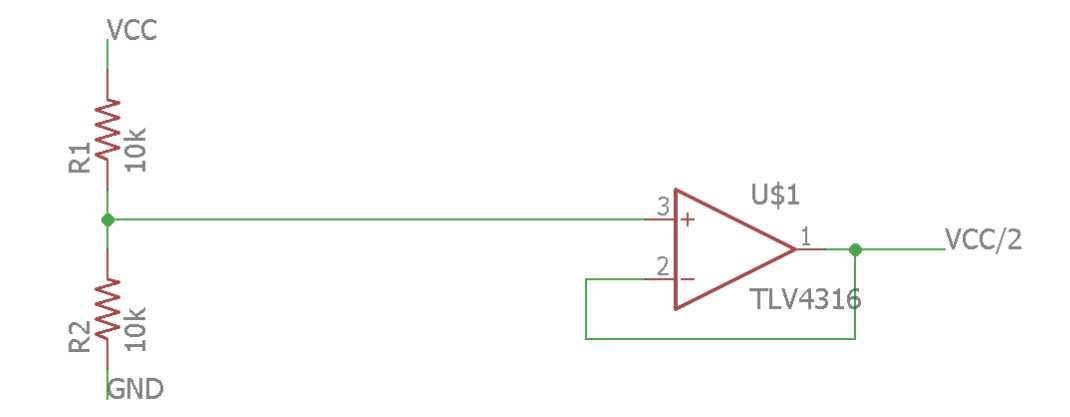
\includegraphics[scale=0.3]{images/virtual}
\legend{Source: made by authors}
\end{figure}

After verify some topologies it was chosen the \textit{inverting signal topology} \cite{OpAmps} as showed on \autoref{Inv_amp}, because it was one of the most simple topologies, the
gain is only on the AC component, because the coupling capacitor on the input prevents the DC gain, so the signal don't presents
DC offset.

\begin{figure}[!htpb]
\centering
\caption{Inverting Amplifier Circuit}
\label{Inv_amp}
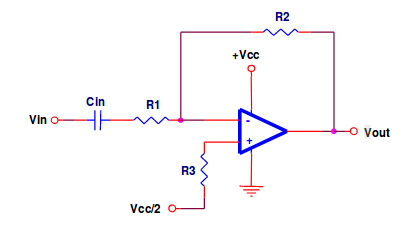
\includegraphics[scale=1]{images/TLV_Gain}
\legend{Source: \citeonline{OpAmps}}
\end{figure}

On this circuit the gain is given by \autoref{TLV_Gain} as verified on the \textit{supplier catalogue} \cite{OpAmps}

\begin{equation}
\label{TLV_Gain}
G=\frac{-R_2}{R_1}
\end{equation}

It is important to verify $R_3$ value, because this resistance value is responsible for bring the error caused by the
input bias current to the minimal value. The relation to verify this value is as showed on \autoref{R3} verified at
the \textit{supplier catalogue} \cite{OpAmps}

\begin{equation}
\label{R3}
R3=R_1||R_2
\end{equation}

It was projected the \textit{schematic circuit} \autoref{TLV_Sch} to perform some simulation tests and verify that the circuit attends the project
requirements. On this circuit, as on the INA one, it was used trimmer potentiometers to be possible perform some precision adjust on the way to have
the best relation on the gain. The schematic project was done using the software CadSoft Eagle Professional 7.6.0 until the final version, as the INA
Schematic project.

\begin{figure}[!htpb]
\centering
\caption{TLV Schematic for 1 channel}
\label{TLV_Sch}
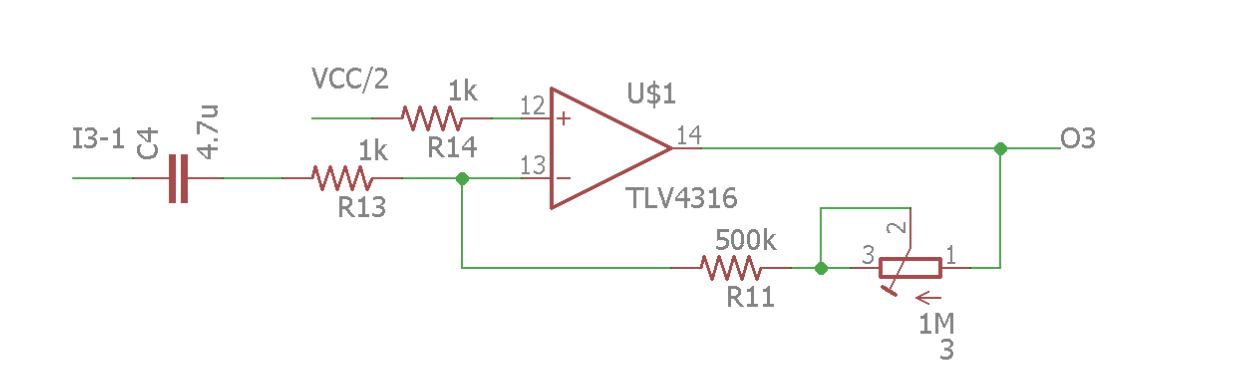
\includegraphics[scale=0.4]{images/TLV_1ch}
\legend{Source: made by authors}
\end{figure}

On this circuit is possible to adjust the gain to near of 100, calculating based on \autoref{TLV_Gain}, adjusting the trimmer potentiometer to the desirable value.\\

It was decided to assembly a usable analogical output, which should sum all the signal of the channels and send to the output, the same function as the monophonic pickups which gets
the variation of all the six strings and transform the harmonic wave into the electric signal. To mount this circuit it was verified the \textit{Inverting Summing Circuit} \cite{OpAmps},
which sums all the input signals. It was assembled the \textit{Summer Circuit Schematic} \autoref{Sum_Sch} based on the circuit presented on \autoref{Sum}.

\begin{figure}[!htpb]
\centering
\caption{Summer Circuit}
\label{Sum}
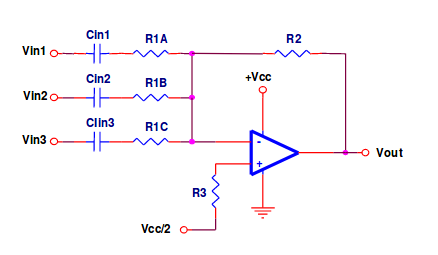
\includegraphics[scale=0.9]{images/sum}
\legend{Source: \citeonline{OpAmps}}
\end{figure}

\begin{figure}[!htpb]
\centering
\caption{Summer Circuit Schematic}
\label{Sum_Sch}
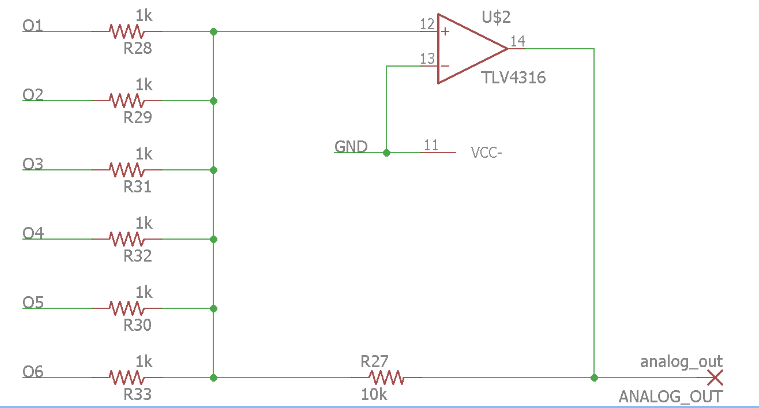
\includegraphics[scale=0.4]{images/tlv_sum}
\legend{Source: made by authors}
\end{figure}

These three parts, virtual grounding, amplifier circuits, summer circuits, compose the \textit{entire schematic} \autoref{TLV_Complete} for the TLV4316 project. It was used the TLV4316 instead the other IC of the family
because it has 4 Operational Amplifiers encapsulated on the same IC, on the project it was used 8 Operational Amplifiers (One on the virtual grounding; Six on the Amplifier Circuits; One on
the Summer circuit).\\

After verify the functionality of the circuit it was projected the \textit{PCB} \autoref{TLV_PCB}, using the same software as the Schematic project. The board was project on dual layer
scheme, using 15 mils of minimum width for the conductive tracks as on the INA PCB project \autoref{INA_PCB_doc}. It was assembled on FR4 dual layer copper
board, combining the through-hole and surface-mount technologies. This choice follows the same reasons as the INA PCB Project which is
the facility of the assembly of the through-hole components and the availability
of the IC only on surface (SOP-8) encapsulation. It was sent
the files to one person who works with printing PCB boards. After the processes
the PCB was like showed on \autoref{TLV_board}.\\

To this project it was used the following component list:

\begin{itemize}
\item 2 Operational Amplifiers TLV 4316;
\item 6 1M$\Omega$ Trimmer Potentiometer;
\item 6 4.7$\mu$F Ceramic Capacitor;
\item 3 10k$\Omega$ $\frac{1}{4}W$ 5 Percent Tolerance Resistor;
\item 18 1k$\Omega$ $\frac{1}{4}W$ 5 Percent Tolerance Resistor;
\item 6 500k$\Omega$ $\frac{1}{4}W$ 5 Percent Tolerance Resistor;
\item 1 6 positions Pin bar;
\item 1 12 positions dual track Pin bar;
\item 1 2 positions Pin bar;
\item 1 1 positions Pin bar;
\end{itemize}

\begin{figure}[!htpb]
\centering
\caption{Projected TLV PCB}
\label{TLV_PCB}
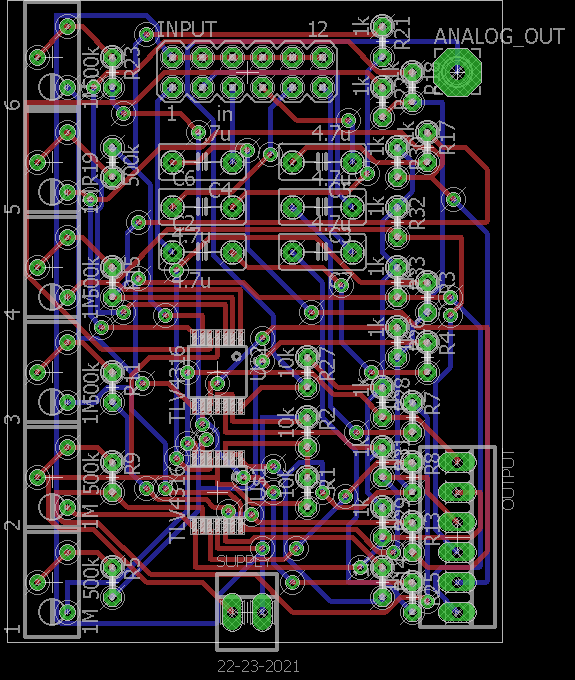
\includegraphics[scale=1.5]{images/tlv_b}
\legend{Source: made by authors}
\end{figure}

\begin{figure}[!htpb]
\centering
\caption{TLV Project}
\label{TLV_board}
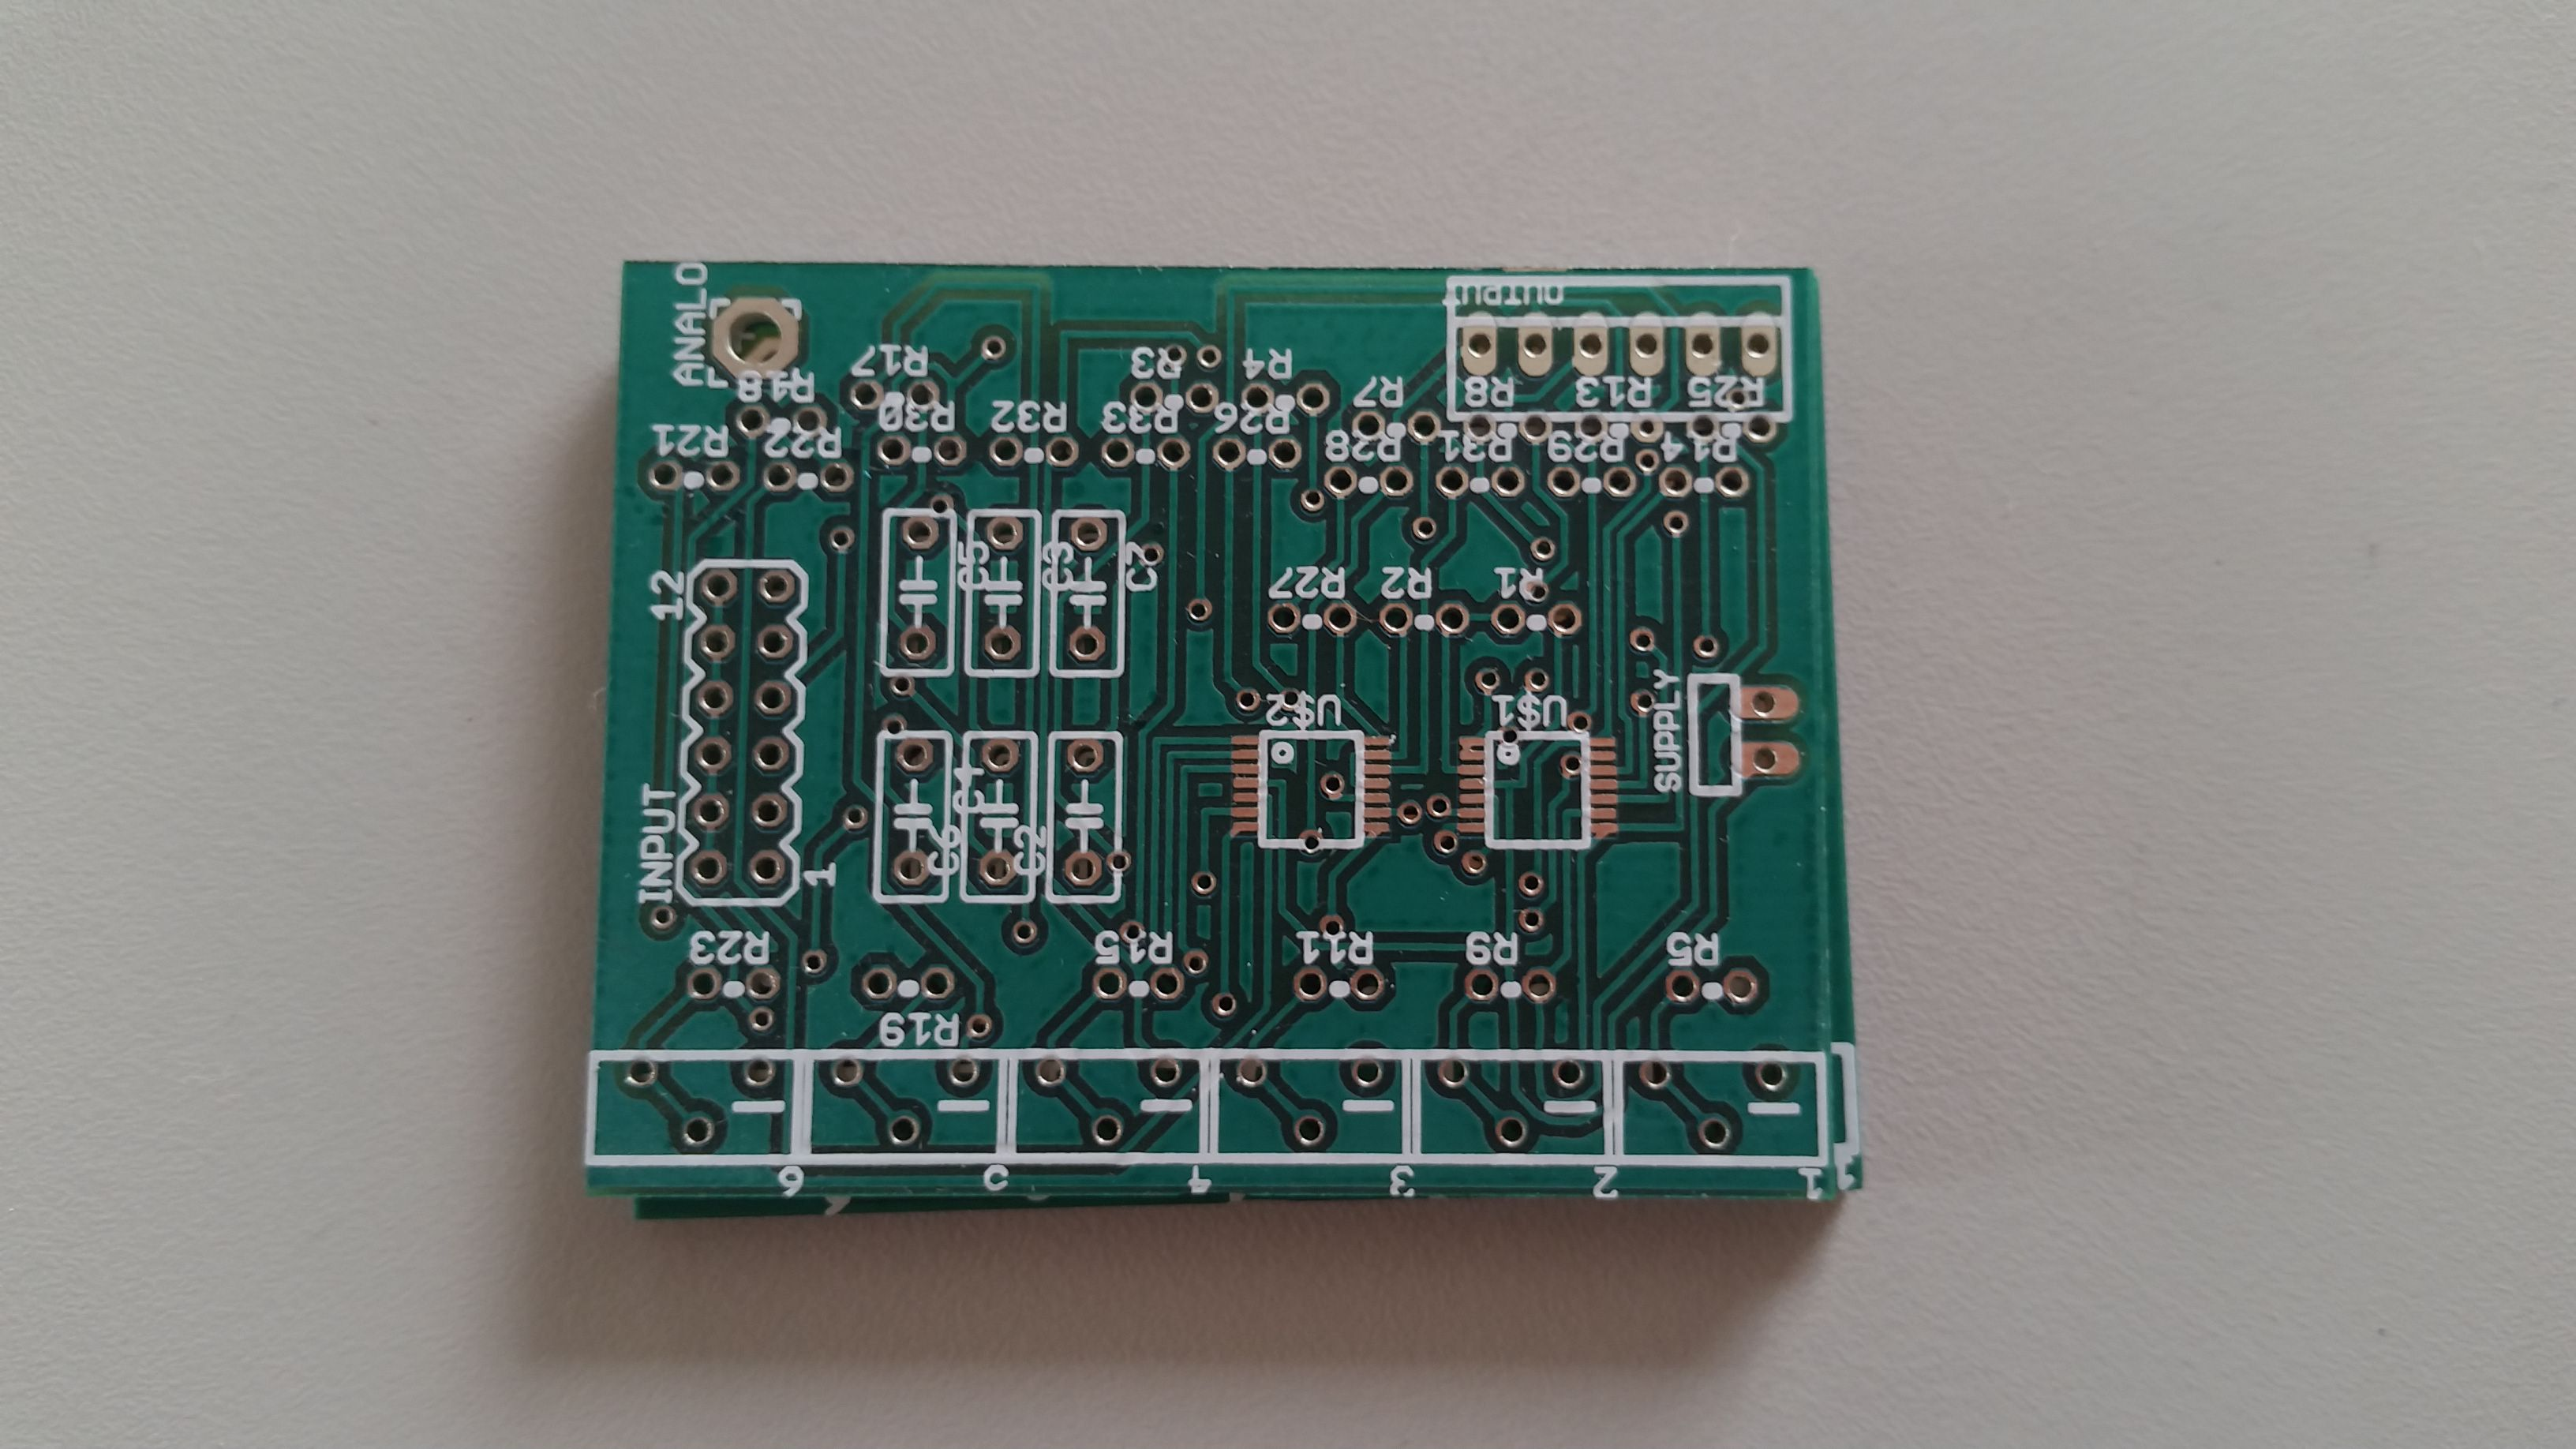
\includegraphics[scale=0.08]{images/TLV_board}
\legend{Source: made by authors}
\end{figure}

After soldering the components it was performed some bench tests to
verify the functionality of the amplifier circuit. The result showed that the
circuit attends the required function, amplifying the signal from a pick of 10mV
to a pick of 1V, proving that the circuit is working perfectly and attending the
demand of the project. After the bench test the system was connected to the pickup
to verify if the guitar signal would be amplified as needed to the conversion process.
The result was satisfactory and attended well the purpose to the project, as showed on \autoref{TLV_result}.

\begin{figure}[!htpb]
\centering
\caption{Amplified pickup signal with TLV circuit}
\label{TLV_result}
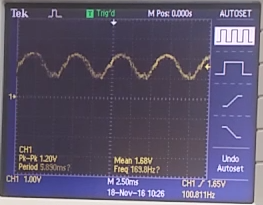
\includegraphics[scale=1]{images/TLV_result}
\legend{Source: made by authors}
\end{figure}

\section{Results}
After assembly both circuits, the \textit{INA Circuit} \autoref{INA_Circuit} and the \textit{TLV Circuit} \autoref{TLV_Circuit},
and perform some analysis on the scope results it was decided to continue the project using the \textit{INA Circuit} \autoref{INA_Circuit}
because it showed a better and consistent response on the amplify process. Comparing \autoref{INA_result} and \autoref{TLV_result}
it is clear that to the same sound frequency the TLV amplifier circuit presents much more noise than the INA circuit, which the signal is really
clear of interferences.
